\section{Key economic concepts \label{sec:econconceptsintro}}

\begin{comment}
Things to get into this section
%===============================

WUD 24 Write up EoS properly!

%maybe for intro
p.2	Single framework for describing different sectors. Examples: food sector, more land intensive? Cf. Isard on no need for separate methods.


WUD 25 -	Equilibrium section. no u'=0 assumptions. No intrinsic reason for thinking abm more accurate but also no reason to reject out of hand. Cf. u'=0 needs cardinal utility.
Need to write this up! One of those things I'll only fully get when I do.
WUD 44	Externalities as the ``villain of the piece.''


%mentioned in market structure
%WUD 48	Entry/exit of firms: so important to GE. What do I need to know about it?

Factors, a little stuff on stocks and flows.
WUD 41	Have I nailed stocks and flows, and how I want to use them? In economics, a flow is just a stock over time - or more precisely the time derivative of a stock.

Backyard production - cross-ref space nuts n bolts intro

%cf. needing some base for comparison for change
%Could be that this goes into later chapter on nuts and bolts
Numeraire versus money. Must mention some basic money points.
FDA 6	Some quotes from beanworld on understanding the meaning of money in the model. May be useful, but I need to update. See beanworld bits below too. 
%cf 2
FDA 3	Actors: finite amount of time, this is what they're optimising fundamentally. Opportunity cost of time.
Don't think you can endogenise Engel's law, though cf. ref that argues you can.
FDA 6	Blaug, where he notes assumptions about constant purchasing power can't be held to be static if "every change in the price of x unaccompanied by an opposite change in some other price alters the value of money." [Econ theory 335]
So, ties to e.g. that you can't entirely separate PED and IED in small economies. Which can be a pain, of course.



Engels law refs. FDA3 p.1
FDA 7	Whole write-up on food an elasticities. Should use.
FDA 7	Engel's law generalised: all elasticities summing to one, but with wealth increase, diverging demand. But is there any reason to think it'll be spatially interesting?



\end{comment}
%===============================

\subsection{Utility \label{sec:utilityintro}}

%Both utility and firm production can be described using the same mathematical tools, and often are. Some of the most common of these are used in parts of this thesis, and they are outlined in this section. The kind of production function used in simple models tend themselves to be simple; generally, `tractable' wins over `realistic': a black box approach where inputs are clearly defined through an equation into some single output. 

At its simplest, utility is a very effective way of describing when an economic actor is better or worse off. It can abstract away from any details about the nature of `better off' in any psychological sense. This is a strength of utility theory, though it is often portrayed as a weakness. Chapter \ref{chapter:ABM} examines these arguments in more depth, since they impact on the way that agent modellers have chosen to approach economics. 

As with \gls{ge}, the forms of utility used here are all reasonably simple and tractable. The simplest of these is the Cobb Douglas. A consumer gets utility from two goods, labelled $F$ and \textbf{$M$.} (For consistency, the variable names here are the same as those used later when discussing geographical economics.)

\begin{equation}
U=F^{a}M^{b}\label{eq:-1}
\end{equation}

The sum of $a$ and \textbf{$b$} control the effect of scale. Summing the exponents to one gives constant returns to scale, whereas if $a+b>1$, the function has increasing returns (see section \ref{sec:prodfuncts} for a full explanation). Most commonly it is assumed that, for utility, $a+b=1$. For this, an equivalent function can be used:

\begin{equation}
U=F^{\delta}M{}^{1-\delta},(0<\delta<1)\label{eq:-3}
\end{equation}

This Cobb Douglas is particularly popular because of the convenient relationship that exists between a consumer's budget and the optimal mix of $F$ and \textbf{$M$. }Let $Y$ be the consumer's budget. Assuming the cost of both $F$ and \textbf{$M$} is unity (they both have a price of one), total consumption cannot be more than the budget:  

\begin{equation}
F+M=Y\label{eq:-2}
\end{equation}

What, then, is the optimal mix of the two goods for the consumer? Maximising \ref{eq:-3} with the budget constraint \ref{eq:-2} gives -

\begin{equation}
F=\delta Y\label{eq:cobbd_optF}
\end{equation}


\begin{equation}
M=1-\delta Y\label{eq:cobbd_optM}
\end{equation}

\begin{figure}%
\centering
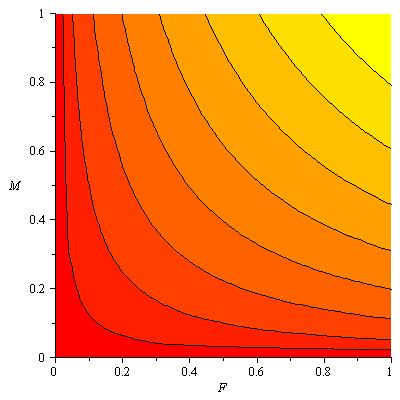
\includegraphics[width=0.3\columnwidth]{ChapterEcon/figures/cobbdouglascontour}%
\caption{Cobb Douglas function, $\delta$ is $0.5$. Contour lines show isoquants.}%
\label{fig:cobbdouglascontour}%
\end{figure}

The Cobb Douglas exhibits, in the simplest way possible, a basic feature used by \gls{ge}: \gls{lov} - a mix of the two goods is preferable to either good alone; see below for a fuller description of this concept. The optimum mix can be controlled with $\delta$, which can be referred to as the 'share parameter'. Figure \ref{fig:cobbdouglascontour} shows contour lines when $\delta=\frac{1}{2}$, indicating isoquants: lines of equal utility, where a consumer would be indifferent between the mix of $F$ and $M$, if their budget didn't matter. However, the budget does: according to \eqref{eq:cobbd_optF} and \eqref{eq:cobbd_optM}, their optimal choice if $\delta=\frac{1}{2}$ is equal. That is, $F=M$ - a positive, straight line. So, for example, if the budget $Y=10$, their utility-maximising mix would be five for each good. These preferences would also be homothetic - if the budget changes, the proportionate mix of optimal goods remains the same: $F$ always equals $M$. (For a fuller outline of constrained optimisation for this and other functions in this section, see appendix \ref{apx:maths}.)

The strength of this simple function, then, is that $\delta$ can so easily be used to find the optimal mix of two goods given any budget. The next section looks at a slightly altered Cobb-Douglas where income level does matter.

\subsection{Utility and Engel's law: the `Engel function' \label{sec:utilitynengelslaw}}

%WUD 14	Readings for Engels law write-up
%WUD 16	Why is Engels law stuff even in here? Haven't justified. Simplest way to illustrate product differentiation?

The next utility function is much less commonly used. It was recently employed by Murata in a \gls{ge} context (\citealt{murata_rural-urban_2002}, \citealt{murata_engels_2008}) and it describes in as simple a way as possible the notion of 'Engel's law' - hence, here it will be described as the 'Engel function'. As Murata puts it, Engel's law is the observation that as incomes increase, ``the expenditure share of food tends to decline, whereas the expenditure share of manufactured goods tends to rise.'' (p.1) Engel's law is an empirical example of demand relations described more generically by Zimmerman as ``the proportionate distribution of expenditures under conditions of increasing or decreasing income'' (\citealt{zimmerman_ernst_1932} p.80). Murata cites the example of Japan, where the expenditure share of food went from 62\% in 1920 to 23\% in 2001. Along with that shift, the employment share of the agricultural sector went from 54\% to 5\% between the same years (\citealt{murata_engels_2008} p.161). 
%the effect of wealth increases on the distribution of expenditures

These kind of income effects are usually avoided by using homothetic functions (like the Cobb Douglas) where wealth increases are matched by proportional demand increases for all goods equally, as this keeps analysis simpler. The most basic version of the Engel function differs from the Cobb Douglas in only one respect - the addition of a variable to control which good is a `necessity' and which a `luxury'. Before getting onto this basic utility function, an outline of the economic meaning of `necessity' versus `luxury' will be useful. Its meaning relates to how `the effect of wealth increases on the distribution of expenditures' is defined. This is done using the \gls{ied} -

\begin{equation}
IED=\frac{\triangle q}{\triangle i}
\end{equation}

 - where $\triangle q$ is the change in quantity demanded and $\triangle i$ is the change in income. It can be seen that, if $0>IED<1$, the quantity of a good demanded, while still increasing, is doing so more slowly than income. It is income inelastic: this is the definition of a necessity good. Where $IED>1$, the change in quantity demanded must be larger than the change in income - this is a luxury good. Note also that, if $IED<0$, it is an `inferior good'. As income increases, demand actually drops.
%Just checked I had my terms right! http://economics.about.com/cs/micfrohelp/a/income_elast.htm
 
In theory, from the point of view of all goods in aggregate, total IED in an economy must be one, since all income will be spent.
\cmt{total ied=1: do I want/need a fuller explanation of that? Not sure.}

Returning to the Engel function, here is its simplest definition:

\begin{equation}
U=F^{\delta}(M+\gamma){}^{1-\delta},(0<\delta<1),\gamma\geq0\label{eq:engelsmurata}
\end{equation}

\begin{figure}
  \centering
 %\subfloat[A gull]{\label{fig:gull}\includegraphics[width=0.3\textwidth]{gull}}                
  %\subfloat[A tiger]{\label{fig:tiger}\includegraphics[width=0.3\textwidth]{tiger}}
  \subfloat[$\delta=0.5$, $\gamma=1$]
  {\label{fig:engel1}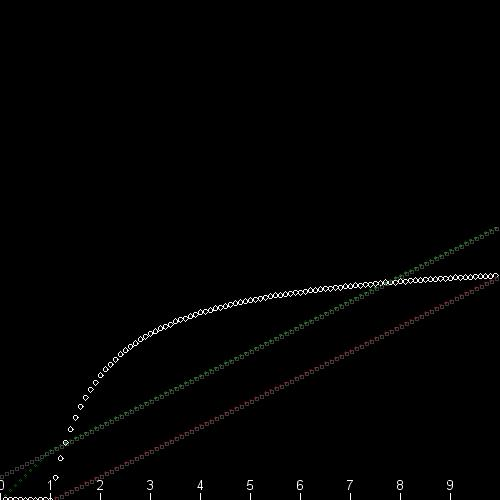
\includegraphics[width=0.3\textwidth]{ChapterEcon/figures/engelsmurata_gamma1_delta05}}
  \hspace{0.2}     
  \subfloat[$\delta=\frac{1}{3}$, $\gamma=2$]
  {\label{fig:engel2}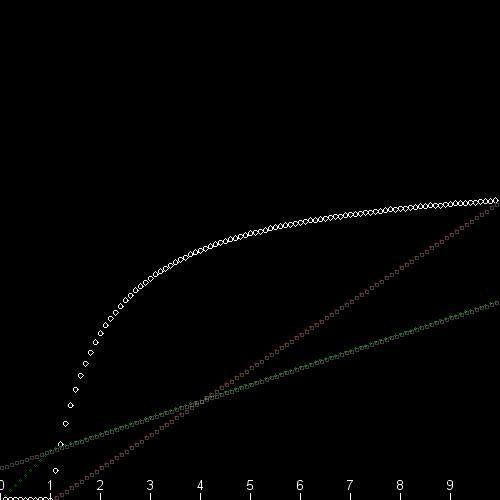
\includegraphics[width=0.3\textwidth]{ChapterEcon/figures/engelsmurata3}}
  \hspace{0.2}  
  \subfloat[$\delta=0.5$, $\gamma=0$]{\label{fig:engel3}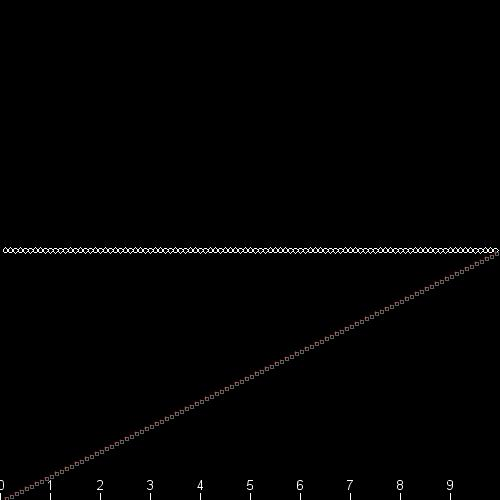
\includegraphics[width=0.3\textwidth]{ChapterEcon/figures/engelsmurata_cobbd}}
  \caption{Engel function showing optimal mix of two goods, one necessity, one luxury for two sets of values of $\delta$ and $\gamma$. Also, with $\gamma=0$, becomes Cobb Douglas (\ref{fig:engel3}).}
  \label{fig:engelfunctionProc}
\end{figure}

So, $\gamma$ controls `the effect of wealth increases on the distribution of expenditures' between the two goods. The optimal quantity of $F$ and $M$ are both positive, straight lines: they are both normal goods where demand increases as income does. The Engel function allows control of the \emph{proportionate changes} in demand for the two goods. If $\gamma$ is zero, the function just becomes the Cobb Douglas. For values above zero, $M$ becomes a luxury good. For instance, consider figure \ref{fig:engelfunctionProc}, a composite of two plots. The straight lines indicate the absolute optimal amount of $F$ (green) and $M$ (red) demanded at a particular budget point, $Y$. The `budget level' from zero to ten is on the horizontal axis. (Again, both goods' cost is unity in this example, so the `budget' is actually the maximum raw quantity of the two goods combined.) The curved line shows the optimal mix of each good for a given budget level: the bottom of the graph indicates necessity good. It can clearly be seen that as the budget increases, the optimal mix approaches an even split, but favours the necessity good at lower budget levels. Here, $\delta$ is 0.5 and $\gamma$ is 1. At this value of $\delta$, $\gamma$ controls where $M$ crosses the x axis. The economic interpretation is that, up to that budget level, there is no demand at all for $M$.

\cmt{Figure \ref{fig:engelfunctionProc}: need to label all axes; only the budget line at the bottom is currently labelled. Curved line: bottom of graph indicates optimum is necessity good; moving towards the top indicates more luxury good is optimal. Straight lines are total good quantities, on different scale.}

$\delta$ itself cannot quite be interpreted as a 'share parameter', as it is for the Cobb Douglas. In combination with $\gamma$, however, it can be used to control the proportionate change in demand as incomes increase. For example, in figure \ref{fig:engel2}, $\delta=\frac{1}{3}$ and $\gamma=2$. While, as $Y\rightarrow\infty$, $\delta$ does indeed describe the final budget share between the two goods, at lower budget levels it also controls in what way proportionate demand for the two goods changes. This can be seen as the two total good demands crossing at the point where the share of $Y$ between $F$ and $M$ passes the half-way mark.

At points below where $M$ has yet to enter into demand in the two figures above, there are two lines. Why is this? The graph actually contains two separate outputs describing the same thing. One is the pair of analytically deduced equations from constraining the Engel function with the simple budget used above, $F+M=Y$. The second is from a brute-force computation of the optimal mix. The Lagrangian produces the following two lines, which both reduce to the Cobb Douglas optima when $\gamma=0$. (In appendix \ref{apx:maths}, this is used as an example to run through Lagrangian optimisation.) 

\begin{equation}
F=\delta(Y+\gamma)\label{eq:engelsmurataFopt}
\end{equation}

\begin{equation}
M=Y-\delta(Y+\gamma)\label{eq:engelsmurataMopt}
\end{equation}

The computational and analytic results are identical, except for values below where \eqref{eq:engelsmurataMopt} crosses the x axis into negative values. 

\cmt{EngelsMurata optimisation: I think I need to leave this discussion until I know how others actually deal with negative values.}

While the Engel function is a fantastically simple way of modelling Zimmerman's `effect of wealth increases on the distribution of expenditures', it has a drawback related to its being non-homothetic. \cmt{non-homothetic cf. Love, 'quasi-homothetic.' Is this right?} To see why, compare to a consumer living in a Cobb Douglas world. For them, it would not make any difference when they consumed their optimal mix of goods - spending twice as much now achieves the same utility as spreading it over two days. Let the budget $Y=2$: what happens if that is spent on two separate occasions, or all at once? For optimal quantities in the Cobb Douglas, use equations \eqref{eq:cobbd_optF} and \eqref{eq:cobbd_optM}: obviously, $F=2\delta$ is the same as $F=\delta+\delta$. Also $M=2(1-\delta)$ is the same as $M=(1-\delta)+(1-\delta)$. Not so for the Engel function's optima, \eqref{eq:engelsmurataFopt} and \eqref{eq:engelsmurataMopt}. A one-day spend of a budget of 2 gives $F=\delta(2+\gamma)=2\delta+\delta\gamma$, whereas a two day spread gives $2(\delta(1+\gamma))=2(\delta+\delta\gamma)=2\delta+2\delta\gamma$. Similarly for $M$, the presence of $(Y+\gamma)$ alters the optimal outcome depending on how a particular budget $Y$ is spent.

Is this a problem? An uncharitable interpretation suggests yes. The Engel function, one might argue, would allow a consumer to increase their total utility merely by buying once in the morning and once in the afternoon. More leniently, it means that the effect of timing must be consciously considered if the Engel function is to be successfully used: how do budgets and time relate to each other?
\cmt{intertemporal utility: another large theory area I need to somehow not step on too much.}

%%%%%%%%%%%%%%%%%%%%%
% CES
%%%%%%%%%%%%%%%%%%%%%

\subsection{The CES function and `love of variety' \label{sec:CESbasics}}


%Now, in my margin notes, I've put ``vs `games you can play with CES functions' '' - presumably to sarcastically draw attention to the contrast here. An avowedly narrow model - general, in the sense of 'whole world', but still narrow. Is the engine up to the job?

%It is worth examining how this was approached, and comparing to the use of another function that pre-dates the CES. The Cobb-douglas function, used earlier by x, can actually be derived as a special case of the CES. It also shares with the CES a first appearance in the literature where comparison to data was a strong motivation for its use. [find.]

\cmt{`it is worth' spending some time checking how often I use the phrase `it is worth'!} 
\Gls{lov} is such a key concept it is worth spending a few moments on the intuition of what it represents. Two identical meals in a row for lunch and dinner, each consisting of a homogenous gloop, is likely to be less satisfying than a good lunch and a three course dinner. At a very different scale, it may also be true that consumers prefer - in aggregate - a choice between four models of car than two, though in total they may buy the same number of cars. 

%The `desirability of variety' is central to Dixit and Stiglitz's 1977 paper on monopolistic competition. 
While the Cobb Douglas does have this dynamic, it is the \gls{ces} function that can best represent it. The \gls{ces} function can control \gls{lov} with a single parameter. First defined by Arrow et al (\citealt{arrow_capital-labor_1961}), it is at the core of \gls{ge} and the \gls{dxs}. It is an economic swiss army knife; ``perhaps the most frequently employed function in modern economic analysis'' (\citealt{durlauf_new_2008} p.737) and is used to represent both production output and utility. The first appearance of the CES function, in its two-input form, saw it being applied to cross-country data. Dixit and Stiglitz give a clear illustration of the basic principle, using a function able to reflect that:

\begin{quote}
``... a consumer who is indifferent between the quantites $(1,0)$ and $(0,1)$ of two commodities prefers the mix ($\frac{1}{2},\frac{1}{2}$) to either extreme.'' (\citealt{dixit_monopolistic_1977} p.297)
\end{quote}

It is easiest to see how this works in a simple two-good function that looks like Dixit and Stiglitz's example, before moving on to the $n$-good case. Consider a consumer with the utility function: 

\begin{equation}
U=\left[F^{\rho}+M^{\rho}\right]^{1/\rho}\label{eq:-4}
\end{equation}

The first thing to note is that, if we suppose $M=0$, and only $F$ has a positive value, then $U=(F^{\rho})^{1/\rho}$. This is always just $U=F$, regardless of the value of $\rho$. If both goods have positive values, and $\rho=1$, this reduces to $U=F+M$ and utility is also entirely linear. But for $0<\rho<1$, the consumer is better off with a mix of the two goods as $\rho\rightarrow0$. So, for example, let $F=4$ and $M=4$. If $\rho=1,$this means utility is just 8. If $\rho=\frac{1}{2}$, however, $F$ and $M$ both become $2$. So utility is then $(2+2)^{2}$or 16 - double the linear result. In effect, $\rho$ is the \gls{lov}. It can also be described as controlling `elasticity of substitution' between goods. For values of $0<\rho<1$, the two goods are imperfect substitutes. This can be seen if the function is altered slightly to:

\begin{equation}
U=\left[\delta F^{\rho}+(1-\delta)M^{\rho}\right]^{1/\rho}\label{eq:-5}
\end{equation}

Again, $\delta$ is a share parameter: the consumer must choose a limited mix of the two goods. Figure \ref{fig:CEStwogoodconstrained} gives an example of the function with an equal amount of each good at the two extremes (four), spreading the share between the two. $\rho$ is $0.5$. This underscores Dixit and Stiglitz's basic point: four of either good alone gives less utility than an even mix, two of each.

There is also only one unique maximum for $\delta$, at 0.5. A consumer is best off with a perfect mix of the two, rather than either extreme (section \ref{sec:constrainedopt} in appendix \ref{apx:maths} gives a more formal derivation showing that the optimal mix is always an even split between the two goods.) This is just a restatement of Dixit and Stiglitz's original point; however the simple principle illustrated here holds for all other versions of the CES. 

\cmt{The Cobb Douglas is a special case of the CES where $\rho=0$. Which is true, but not really easily seen: requires l'opital's rule. Should I mention it?}

\begin{figure}%
\centering
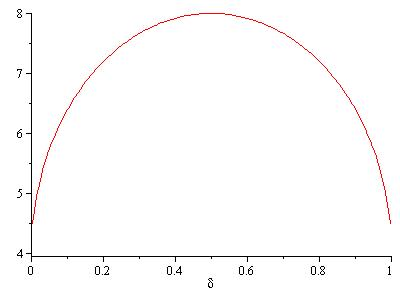
\includegraphics[width=0.5\columnwidth]{ChapterEcon/figures/CEStwogoodstradeoff}%
\caption{Two-good CES function, $\rho=\frac{1}{2}$, constrained by $\delta$, $0<\delta<1$}%
\label{fig:CEStwogoodconstrained}%
\end{figure}

The many-good CES is just an extension of the above: 

\begin{equation}
U=\left(\sum_{i=1}^{N}c_{i}^{\rho}\right)^{1/\rho}\label{eq:-6}
\end{equation}

In this version, $c$ denotes the quantity of good $i$ and can - in theory - be set individually, so that utility is dependent on all goods. This concludes the discussion of utility, except to say that a continuous-varieties version of the CES function is given in section \ref{sec:marketstructure} in the context of \gls{monocomp}.

%%%%%%%%%%%%%%%%%%%%%%%%%%%%%%%%%%%
% Firm and production-related stuff
%%%%%%%%%%%%%%%%%%%%%%%%%%%%%%%%%%%
\subsection{Production, increasing returns and the `law of the minimum' \label{sec:prodfuncts}}

%Once a discussion about the functional structure of utility has been covered, much of the detail of production is also done, since often, firms' output takes the same form as utility. 

Firms' production functions used in this thesis have the same many-to-one functional form ($x=f(a,b,c .. n)$) as utility. The simplest production function has only one input. In the \gls{coremodel}, for example, labour is the only productive factor. The most obvious multi-input function has already been mentioned in section \ref{sec:utilityintro}: the Cobb Douglas first came into being as a production function. 

The vital requirement for getting firms to function in space, however, is economies of scale, or increasing returns. The discussion of market structure in sections \ref{sec:marketstructure} and \ref{sec:marketstructnspace} explains why increasing returns are analytically necessary; this section outlines how increasing returns enter into production functions. For a Cobb Douglas-type function, the simple way to control returns to scale has already been mentioned: whether the sum of the exponents is more or less than one will dictate whether it exhibits increasing or diminishing returns respectively. 

Single-input production functions can use simple equation forms for turning an input into some larger output quantity. The \gls{coremodel} just uses a straight line equation, where output ($x$) is defined in terms of the amount of labour ($l$) required to produce it, and where $\alpha$ are fixed costs and $\beta x$ are variable costs:

\begin{equation}
l = \alpha + \beta x
\label{eq:coremodelMprod}
\end{equation}}

The discussion of this approach is left to sections \ref{sec:spacemaths} and \ref{sec:agenttimings}. Chapter \ref{chapter:ABM} also takes a critical look at this `black box' approach to production functions. 
\cmt{check references for connections to production discussion}



The second function is outlined in section \ref{sec:modelutility_prod}: its job is to provide a smooth transition between backyard and collaborative production and avoid some of the agent-related issues that stem from using equation \eqref{eq:coremodelMprod}. (Section \ref{sec:agenttimings} explains these agent-related problems.)
%Note also the economic assumptions that make marginal analysis viable. Er, like what?

\subsection{The `ecological' criticism \label{sec:ecocrit}}

The kind of production and utility functions described get plenty of criticism, aimed in one way or another at their intrinsic lack of realism. Ecological economics, for example, sees in the Cobb Douglas function a `Garden of Eden' world \fixref{GR quoted in Daly} where natural resources are optional. Daly sums this up nicely, if somewhat loquaciously. He begins by quoting Solow saying, ``if it is very easy to substitute other factors for natural resources, then there is in principle no `problem'. The world can, in effect, get along without natural resources'' (Solow quoted in \citealt{daly_georgescu-roegen_1997} p.261)} Daly responds that economists seem to believe in - 

\begin{quote}
``making a cake with only the cook and his kitchen. We do not need flour, eggs, sugar, etc., nor electricity or natural gas, nor even firewood. If we want a bigger cake, the cook simply stirs faster in a bigger bowl and cooks the empty bowl in a bigger oven that somehow heats itself.'' (ibid.)
\end{quote}

More formally, he quotes Georgescu-Rosen's critique of the Solow-Stiglitz production function - a Cobb Douglas with the addition of natural resources: 

\begin{equation}
Q=K^{a1}R^{a2}L^{a\text{3}}\label{eq:}
\end{equation}

He points out this means that $R^{a2}=Q/K^{a1}L^{a3}$. So, holding labour constant, one could get any quantity of output with a vanishingly small amount of $R$, as long as $R>0$ and $K$ is large enough to compensate for that tiny amount.  Solow's reply to this highlights a recurring argument used to defend the abstract nature of many economic models: critics are taking them too literally, and not considering how the models are used:

\begin{quote}
``We were trying to think about an interesting and important question: how much of a drag on future growth, or even on the sustainability of current production, might be exercised by the limited availability of natural resources and the inputs they provide? ... The role of theory is to explore what logic and simple assumptions can tell us about what data to look for and how to interpret them in connection with the question asked.'' \fixref{(solow p.267/8)}
\end{quote}

Solow goes on to point out that the argument should be about how substitutable renewable and non-renewable resources are, given that the former are likely to be highly capital-intensive. (Ibid.) He appears to be saying that his critics have mistaken economists' models for their actual understanding of the world, rather than tools that aid that understanding. Krugman makes much the same kind of plea. \fixref{krugman, models as aids.} 

\cmt{need to x-ref solow discussion with Friedman stuff. Need to get hold of friedman stuff!}
There are two relevant issues here for the current discussion - one theoretical, the other much more specific to the model work. 
\cmt{Solow, silliness of assumptions, models. Where to write up philosophical? probably not here.}

There is a much more specific point regarding the use of Cobb-Douglas type functions in both production and consumption. If goods are priced near to zero, people with Cobb Douglas-type utility will want to buy increasingly massive amounts. This rules out the use of free inputs - which would be infinitely in demand. In general, the notion of free goods makes no sense in an analytic economic context, so why does this matter? In the models developed here, it transpires that assuming that land can be free to the person using it solves a number of other modelling issues. Most importantly, it removes land from considerations of price. This is discussed in-depth in section x, but -
\cmt{free land discussed where?}

There is a very popular coffee stand at the University of New South Wales that manages an impressive quality and quantity of output through careful division of labour. This could be modelled as a simple production function with increasing returns on labour. But would a Cobb Douglas work, with labour and coffee beans as the two inputs? Following on from Daly's critique, it is clear that increasing the number of coffee beans could not substitute for a loss of workers. Quite the reverse: any increase in output \emph{requires} an increase in beans. Labour input cannot increase without more material input.

\cmt{need some LOTM ref}
A simple way to model this is to use a \gls{lotr}. This simply states that output cannot be more than the minimum input present. In practice, output needs to be defined in relation to each input, since they will not be of the same type. But given that, a function can be defined that will limit the coffee stand's output by whichever is the scarcer of the two inputs, while also allowing for increasing returns.

Returning to the previous discussion, consider a person able to produce using just two inputs: their own labour, and a quantity of land. Using the \gls{lotr} allows a person's output to be limited by one or the other. Whereas, in a Cobb Douglas situation, they could increase their output by inputting more land (while keeping only their own daily labour, say) this approach gives people no incentive to use more land than they can use. If land is actually indivisible and takes up space, and once distance costs are introduced, there is an active \emph{dis}incentive to over-use land. It also allows land to be free.
\cmt{Freeland: a silly assumption. Need to justify why somewhere. Answer: well, I'm conscious of it, and it allows interesting modelling. I need no other reason!}





%%%%%%%%%%%%%%%%%%%%%%%%%%%
% EXTERNALITIES
%%%%%%%%%%%%%%%%%%%%%%%%%%%
\subsection{Externalities \label{sec:externalities}}

External economies and externalities have a central role to play in analytic approaches to understanding agglomeration, and are key to the core model also. The two concepts are connected, but slightly different; as explained in detail below, externalities refer to actual variables appearing in actors' production or utility functions. External economies, in contrast, is a more general term: if a region is said to have external economies, it could be (for instance) that there are economies of scale at the industry level. Looking at externalities first, Button defines them as where - 

\begin{quote}
``... the activities of one group affect the welfare of another group without any payment or compensation being made.'' (Button 2010, p.161) 
\end{quote}

%The idea is so central for modern location theory that 'localisation' and 'urbanisation' externalities are often taken to be synonymous with agglomeration effects. 
%\cmt{vague statement about externalities being synonymous with agglom. Needs backup.}
%Indeed, the spatial equilibria that result in cities and settlements can be said to be nothing more than the balance of positive and negative externalities. 

The concept of externalities is so central because of the role they play in market structure. The pivotal chunk of Button's definition is `without any payment or compensation being made'; externalities are outside of the price system. Scitovsky (\citeyear{scitovsky_two_1954}) first clearly formulated their meaning as `direct interdependence' between economic actors. Scitovsky defined this interdependence in two ways, as technological (or `pure') and pecuniary externalities. The first, technological, he defined in relation to a firm's production function -

\begin{equation}
x_{1}=F(l_{1},c_{1},...;x_{2},l_{2,}c_{2},...)\label{eq:scit1}
\end{equation}

 - where $x_{1}$ is its output (\citealt{scitovsky_two_1954} p.145). $l_{1}$ and $c_{1}$ are its own inputs. By including a second firm's output ($x_{2}$) and its inputs ($l_{2}$ and $c_{2}$), Scitovsky explicitly states the interdependence: any alteration in the second firm's outputs or inputs will impact on the output of the first, changing the technical relations in its own production function. It is more common in spatial settings for externalities to be considered as an aggregrate effect within a region; for example, in Brakman \emph{et al} (p.38), where ``an increase in \emph{industry-wide} output alters the technological relationship between inputs and output for each individual firm. It therefore has an impact on the firm's production function'' (emphasis added). The result is the same: a firm's production function is dependent not only on the inputs it buys, but the actions of other firms. Early on, Scitovsky pointed out the rarity of this kind of `pure' externality: 

\begin{quote}
``It is not easy to find examples from industry. Going through the many examples of external economies quoted in the literature, I found only two that fit the above definition: the case in which a firm benefits from the labour market created by the establishment of other firms and that in which several firms use a resource which is free but limited in supply.'' (p.145) 
\end{quote}

Examples of the latter he gives are all common pool resources: production changes from oil-well drilling of others; fishermen using the same waters; congestion problems on a public road. In a sense, even labour market pooling can be seen as a common-pool resource.

Moving on to the second type, in similar fashion, Scitovsky defines pecuniary externalities in relation to a firm's profits \citealt{scitovsky_two_1954} p.146):

\begin{equation}
P_{1}=G(x_{1,}l_{1},c_{1},...;x_{2},l_{2,}c_{2},...)\label{eq:scit2}
\end{equation}

These profits are, of course, a function of its output and inputs, but also of other firms'. These affect the \emph{profits}, however; they do not alter the production function. Scitovsky's example of a pecuniary externality is a firm investing to increase its efficiency. The investment gives it better economies of scale; it can sell its output for less. This also means inputs to the firm increase - this is where a pecuniary externality can be found. That increase in demand will push the price of that input up. For other firms using it, that is a negative externality. For any firms selling it, it is positive (Scitovsky p.149).

Scitovsky points out that externalities are - for general equilibrium theory and many arguments about market structure - ``the villain of the piece and the cause for conflict between private profit and social benefit'' (\citealt{scitovsky_two_1954} p.144). One of the key elements of \gls{ge}'s success stems from having managed to combine externalities and equilibrium in a way that avoids this apparent villainy. The next section starts to explain why market structure is so important to this argument.

%%%%%%%%%%%%%%%%%%
%	MARKET STRUCTURE
%%%%%%%%%%%%%%%%%%
\subsection{Market structure \label{sec:marketstructure}}
%putting CES and monopcomp in the context of market structure, and why it became popular

The way in which market structure has been theorised lies at the heart of how space has come to be modelled in \gls{ge} and elsewhere. Its relation to space is covered in more depth in section \ref{sec:marketstructnspace}; this section looks at the relevant economic aspects.

There are three broad categories of favoured market structure in analytic economics: perfect competition, monopoly and monopolistic competition. Why `favoured'? Each of these are analytically tractable and (relatively) simple. Perfect competition and monopoly have straightforward mathematical interpretations: in the former, the size of the market is so large that no one economic actor can affect price: everyone is assumed to be a `price-taker'. In practice this means prices can be treated as constants. (This is generally the case, though general equilibrium theory has developed an argument for perfect competition that does not rely on assuming all actors are price-takers; see e.g. \citealt{starr_general_1997} pp.157.) Not only does this mean consumers can have no effect on price, but firms cannot either - and so strategic interaction is ruled out. In a monopoly, on the other hand, the monopoly firm can set a price that gives them the best revenue, based on the supply-demand curve they face for their product. Again, there are no other firms, so they face no strategic considerations, and the revenue-maximising calculation is straightforward.

%%%%%%%%%%%%%%%%
%Discuss economies of scale in 'firms and production functions.'
Perfectly competitive models must work with linear output - no increasing returns are allowed. To see why, consider a (rather artificial) situation where many firms have linear output, but one firm, producing the same good, is able to utilise economies of scale. They can thus produce each unit more cheaply than their competitors - and so this is no longer a perfect competition situation. A single price can no longer be assumed, nor can one say that no actor can influence price. In this case, that one firm can immediately gains monopoly power (assuming they can access inputs to meet demand.)

Between these two poles, a sprawling tangle of approaches to imperfect competition has been developed over the twentieth century. This tangle helps to explain why the publication of the \gls{dxs} is such a pivotal moment in the history of market structure models. The \gls{monocomp} model first published by \citeauthor{dixit_monopolistic_1977} in 1977 is one of the most prominent approaches to imperfect competition; it is also the `engine' of \gls{ge}. As Brakman \emph{et al} note, in providing a tractable method able to do away with many of the complexities facing theorists of imperfect competition, it neatly sidesteps ``getting bogged down in a taxonomy of oligopoly models'' (\citealt{brakman_new_2009} p.93). In particular, it can account for economies of scale, and it finds a way around problems of strategic interaction.

Fujita, in his recent short history of spatial economics, makes some strong claims for the \gls{dxs}: von Thunen could not have produced anything other than the partial theory he did, any more than one could expect ``de Vinci, upon one's first view of his amazing `flying machines' drawn in the fifteenth century, to invent a real airplane'' without access to the internal combustion engine. For Fujita, the \gls{dxs} ``provided location theory with a powerful combustion engine.'' (\citealt{fujita_evolution_2010} p.8) That engine drives the \gls{coremodel} of \gls{ge}.

Section \ref{sec:spaceconceptsintro} deals with how the \gls{dxs} found its way into a spatial setting. Here, the basic principles of the approach will be covered, insofar as they are relevant to understanding the spatial analysis. The starting point for Dixit and Stiglitz has already been outlined in discussing the \gls{ces} function. That section explained how the CES can be used to describe an `optimum product diversity' from a utility point of view. 

%%%
\begin{figure}%
\centering
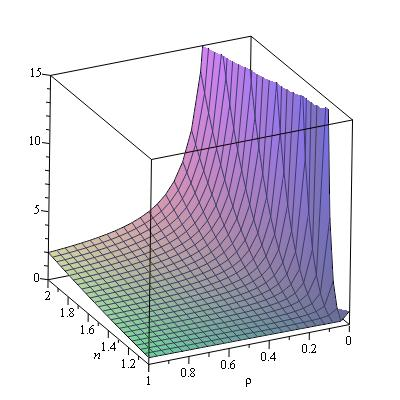
\includegraphics[width=0.5\columnwidth]{ChapterEcon/figures/integralCES}%
\caption{Continuous CES function, $0<\rho<1$, $1<n<2$}%
\label{fig:CESintegral}%
\end{figure}

Perhaps the most central simplification of the \gls{dxs} is the assumption that goods enter symmetrically into demand. As Fujita \emph{et al} note, this ``lets us have our cake in discrete lumps while doing calculus on it, too'' (\citealt{fujita_spatial_2001} p.7). What this means in practice is that, in the many-good CES function \eqref{eq:-6}, all $c_{i}$ have the same value. Sometimes, this is guaranteed mathematically by defining it as an integral (see e.g. \citealt{fujita_spatial_2001} p.46), where $n$ is the (now continuous) number of varieties, and $m(i)$ stands in for the consumption of each variety:

\begin{equation}
M=\left[\int_{0}^{n}m(i)^{\rho}di\right]^{1/\rho}\; 0<\rho<1\label{eq:integralCES}
\end{equation}

It helps to get a quick visualisation of what this means by reframing \eqref{eq:integralCES}, assuming one unit of each variety:

\begin{equation}
M=\left[\frac{n^{\rho+1}}{\rho+1}\right]^{1/\rho}\label{eq:integralCESsimplified}
\end{equation}

Recall that $\rho$ controls \gls{lov}: the closer to zero, the more variety is preferred. If the number of varieties ranges from one to two, $\rho$ looks like figure \ref{fig:CESintegral}. As $\rho$ approaches zero, increasing \gls{lov}, and as the number of varieties $n$ increases, $M$ increases. Where $\rho=1$ it can be seen that $M$ increases linearly with $n$. 

\cmt{behaviour of this function below one is peculiar, nothing like $>1$. Not seen this mentioned anywhere. Is this a problem? Have I got the basic point right?}

%explain what M is, output from firms is in there (n), but it's utility from that. Except it isn't, it's actually output from firms. That's odd, isn't it? cf. Brakman and crit of this approach. 
In terms of market structure, the \gls{dxs} can guarantee that each firm only produces a single variety. Increasing returns take care of that: any firm producing one good will be locked in to producing it more cheaply than any other can. As a firm, it is always better to devote all of one's resources to that single product than attempt to split over more than one, since this allows full exploitation of increasing returns, and thus one's market power. This is an assumption that the thesis sticks to, though in section x, it will be questioned. 

Because firms are locked into one product, the relation to \gls{lov} means that economies have an equilibrium number of firms, and thus varieties. An argument from perfect competition is utilised: firm profits are set to zero as an equilibrium condition, underpinned by arguing that profits attract firms and losses drive them away. As discussed in section x, this is a particularly thorny problem for agent modelling.
\cmt{basic point is clear; don't know if I need more detail on this. May become important.}

%%%%%%%%%%%%%%%%%%
%	CUTTINZ
%%%%%%%%%%%%%%%%%%
\begin{comment}

\subsection{Cuttings \label{basicscuttings}}

The many-good CES comes in two varieties: discrete and continuous. For the former - 

\begin{equation}
U=\left(\sum_{i=1}^{N}c_{i}^{\rho}\right)^{1/\rho}\label{eq:-6}
\end{equation}

In this version, $c$ denotes the quantity of good $i$ and can - in theory - be set individually, so that utility is dependent on the sum of all goods. However, usually in geographical economics, consumption of each good is symmetric: quantities for each are the same. Given this, a continuous integral can also be used to describe utility:

\begin{equation}
U=\left[\int_{0}^{n}c(i)^{\rho}di\right]^{1/\rho}\label{eq:-7} 
\end{equation}

Here, $n$ is the total range of goods consumed, and $c(i)$ indicates the consumption level, which is symmetric across all goods. This is used in Dixit and Stiglitz's formulation for monopolistic competition (see also Fujta et al 1999 p.46), whereas the discrete version is used more in work related to the core model. Looking at \ref{eq:-7}, the definite integral is just:

\begin{equation}
\int_{0}^{n}c(i)^{\rho}di=\left[\frac{n^{\rho+1}}{\rho+1}\right]_{0}^{n}\label{eq:mcderiv1}
\end{equation}

%%%%%%%%%%%%%%
Models have structural elements that look nothing like the real world, but can be argued to capture some element of it. The CES function in the core model is one such structure: Krugman wants to persuade us that it captures something important about \gls{lov} in the real world. It is easy enough to list the ways in which it is nothing like the real world; however, as noted, \gls{ge} theorists are aware of this, and argue nevertheless for the usefulness of the method. This section looks in more detail at the CES function, and the job it is asked to do in \gls{ge}. 
%%%%%%%%%%%%%%
In analytic approaches to market structure, there is a tight symbiotic relationship between theory structure and the mathematics that describe it. The particular form of market structure is very much determined by mathematical approach, and the \gls{coremodel} is no different. A full survey of the literature on market structure is beyond the scope of this thesis, but it is important to understand the context that led to the creation of the \gls{coremodel}. As well as shedding light on the model itself, arguments about market structure in analytic economics set the scene for discussing agent-based approaches to the same problems. 
%%%%%%%%%%%%%%%
%Before getting into the technical details, it is worth quickly outlining the key role the CES function plays in GE. It begins with Dixit-Stiglitz - ``a formalization of Chamberlin's concept of monopolistic competition that, though admittedly a very special case, has turned into the workhorse of theoretical modelling in a number of fields.'' (\citeauthor{fujita_spatial_2001}, p.3) Because analytically tractable.

%They note that many theorists have attacked the problem, often through `product space' approaches, which they find lack generality. 
%A clear example of this also comes from Krugman's work on international trade, discussed above, and cannot be put better than Krugman himself does in the abstract to his original 1979 paper: 

%\begin{quotation}``... trade, and gains from trade, will occur, even between countries with identical tastes, technology, and factor endowments.'' (Krugman 1979 p.469)\end{quotation}

%Or rather, they will occur in the model that Krugman presents. The model itself cannot guarantee the real world contains the same dynamic; the point is to show that such a dynamic is \emph{possible}, given a particular set of assumptions. 


\end{comment}

